\section*{Figures}

% System Architecture Diagram
% System Architecture Diagram for Biological Countercurvature Framework
% TikZ diagram showing the complete framework

\begin{figure}[h!]
\centering
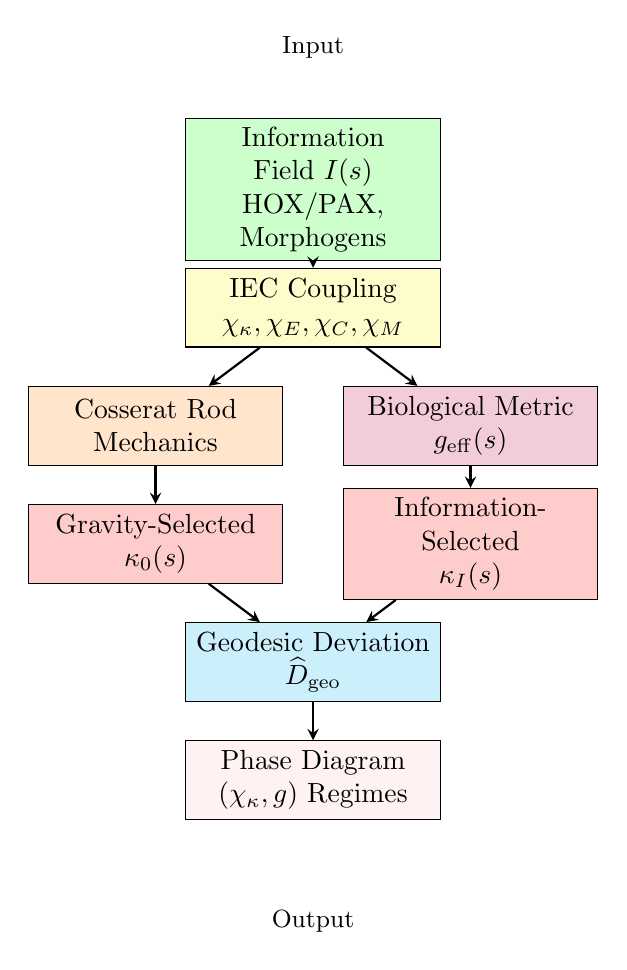
\begin{tikzpicture}[
    node distance=1.5cm,
    box/.style={rectangle, draw, fill=blue!10, text width=3cm, text centered, minimum height=1cm},
    arrow/.style={->, >=stealth, thick},
    label/.style={font=\small}
]

% Information Field Layer
\node[box, fill=green!20] (info) {Information Field $I(s)$\\HOX/PAX, Morphogens};

% IEC Coupling Layer
\node[box, fill=yellow!20, below of=info] (iec) {IEC Coupling\\$\chi_{\kappa}, \chi_{E}, \chi_{C}, \chi_{M}$};

% Cosserat Rod Layer
\node[box, fill=orange!20, below of=iec, xshift=-2cm] (cosserat) {Cosserat Rod\\Mechanics};

% Countercurvature Metric Layer
\node[box, fill=purple!20, below of=iec, xshift=2cm] (metric) {Biological Metric\\$g_{\mathrm{eff}}(s)$};

% Curvature Profiles
\node[box, fill=red!20, below of=cosserat] (kappa0) {Gravity-Selected\\$\kappa_{0}(s)$};

\node[box, fill=red!20, below of=metric] (kappaI) {Information-Selected\\$\kappa_{I}(s)$};

% Geodesic Deviation
\node[box, fill=cyan!20, below of=kappa0, xshift=2cm] (dgeo) {Geodesic Deviation\\$\widehat{D}_{\mathrm{geo}}$};

% Phase Diagram
\node[box, fill=pink!20, below of=dgeo] (phase) {Phase Diagram\\$(\chi_{\kappa}, g)$ Regimes};

% Arrows
\draw[arrow] (info) -- (iec);
\draw[arrow] (iec) -- (cosserat);
\draw[arrow] (iec) -- (metric);
\draw[arrow] (cosserat) -- (kappa0);
\draw[arrow] (metric) -- (kappaI);
\draw[arrow] (kappa0) -- (dgeo);
\draw[arrow] (kappaI) -- (dgeo);
\draw[arrow] (dgeo) -- (phase);

% Labels
\node[label, above of=info, yshift=0.3cm] {Input};
\node[label, below of=phase, yshift=-0.3cm] {Output};

\end{tikzpicture}
\caption{System architecture of the biological countercurvature framework. The information field $I(s)$ (top) drives IEC coupling parameters, which modify both Cosserat rod mechanics and the biological metric $g_{\mathrm{eff}}(s)$. The resulting curvature profiles $\kappa_{0}(s)$ and $\kappa_{I}(s)$ are compared via the geodesic deviation $\widehat{D}_{\mathrm{geo}}$, which maps to countercurvature regimes in the $(\chi_{\kappa}, g)$ phase diagram.}
\label{fig:system_architecture}
\end{figure}



% IEC Equations Diagram
% IEC Equations Diagram
% Visual representation of the IEC coupling equations

\begin{figure}[h!]
\centering
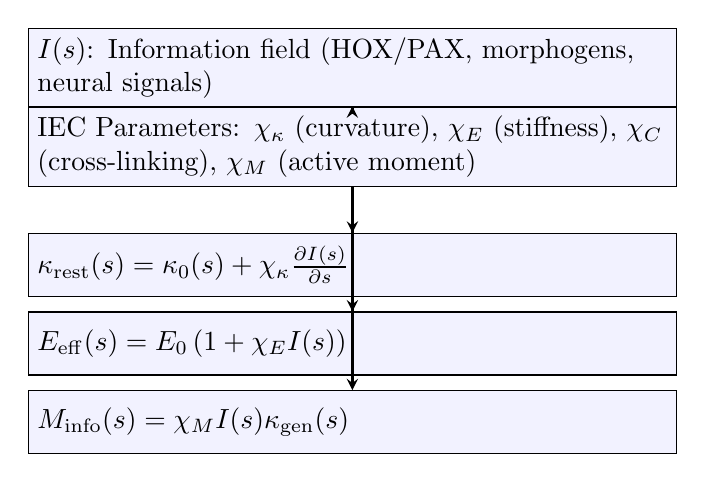
\begin{tikzpicture}[
    node distance=1cm,
    eqbox/.style={rectangle, draw, fill=blue!5, text width=8cm, minimum height=0.8cm, align=left},
    arrow/.style={->, >=stealth, thick}
]

% Information Field
\node[eqbox] (I) {$I(s)$: Information field (HOX/PAX, morphogens, neural signals)};

% IEC Parameters
\node[eqbox, below of=I] (params) {IEC Parameters: $\chi_{\kappa}$ (curvature), $\chi_{E}$ (stiffness), $\chi_{C}$ (cross-linking), $\chi_{M}$ (active moment)};

% Equations
\node[eqbox, below of=params, yshift=-0.5cm] (eq1) {$\kappa_{\mathrm{rest}}(s) = \kappa_{0}(s) + \chi_{\kappa} \frac{\partial I(s)}{\partial s}$};

\node[eqbox, below of=eq1] (eq2) {$E_{\mathrm{eff}}(s) = E_{0} \left(1 + \chi_{E} I(s)\right)$};

\node[eqbox, below of=eq2] (eq3) {$M_{\mathrm{info}}(s) = \chi_{M} I(s) \kappa_{\mathrm{gen}}(s)$};

% Arrows
\draw[arrow] (I) -- (params);
\draw[arrow] (params) -- (eq1);
\draw[arrow] (params) -- (eq2);
\draw[arrow] (params) -- (eq3);

\end{tikzpicture}
\caption{Information-Elasticity Coupling (IEC) equations. The information field $I(s)$ modulates mechanical properties through dimensionless coupling parameters $\chi_{\kappa}$, $\chi_{E}$, $\chi_{C}$, and $\chi_{M}$, producing modified rest curvature, effective stiffness, and active moments.}
\label{fig:iec_equations}
\end{figure}




\begin{figure}[h!]
    \centering
    \begin{subfigure}[b]{0.48\textwidth}
        \centering
        \includegraphics[width=\textwidth]{fig_countercurvature_panelA.pdf}
        \caption{Curvature profiles $\kappa_{0}(s)$ vs $\kappa_{I}(s)$.}
    \end{subfigure}
    \hfill
    \begin{subfigure}[b]{0.48\textwidth}
        \centering
        \includegraphics[width=\textwidth]{fig_countercurvature_panelB.pdf}
        \caption{Countercurvature metric $g_{\mathrm{eff}}(s)$ and information field.}
    \end{subfigure}

    \vspace{0.5em}

    \begin{subfigure}[b]{0.48\textwidth}
        \centering
        \includegraphics[width=\textwidth]{fig_countercurvature_panelC.pdf}
        \caption{Normalized geodesic deviation $\widehat{D}_{\mathrm{geo}}$ vs $\chi_{\kappa}$.}
    \end{subfigure}
    \hfill
    \begin{subfigure}[b]{0.48\textwidth}
        \centering
        \includegraphics[width=\textwidth]{fig_countercurvature_panelD.pdf}
        \caption{Microgravity adaptation: $\widehat{D}_{\mathrm{geo}}$ vs $g$.}
    \end{subfigure}

    \caption{Information-driven countercurvature in spine-like and plant-like configurations.
    Panel A shows the curvature profiles for passive (gravity-only) and information-coupled configurations. Panel B displays the countercurvature metric $g_{\mathrm{eff}}(s)$ along the rod axis, highlighting regions of high information processing. Panel C demonstrates how normalized geodesic deviation $\widehat{D}_{\mathrm{geo}}$ increases with information--curvature coupling strength $\chi_{\kappa}$. Panel D shows that $\widehat{D}_{\mathrm{geo}}$ persists as gravitational loading is reduced, while passive curvature energy collapses, demonstrating information-driven structure maintenance in microgravity.
    }
    \label{fig:countercurvature_main}
\end{figure}

\begin{figure}[h!]
    \centering
    \includegraphics[width=0.65\textwidth]{fig_phase_diagram_scoliosis.pdf}
    \caption{Phase diagram in $(\chi_{\kappa},g)$ showing gravity-dominated, cooperative, and information-dominated regimes. Contours: $\widehat{D}_{\mathrm{geo}}$. Markers: points where a small thoracic asymmetry ($\varepsilon_{\mathrm{asym}}=0.05$) produces a scoliosis-like branch (high $S_{\mathrm{lat}}$ and Cobb-like angles). The scoliotic regime (shaded) emerges in the information-dominated corner where $\widehat{D}_{\mathrm{geo}}>0.3$ and small asymmetries are predicted to be amplified.}
    \label{fig:phase_diagram}
\end{figure}
